\chapter{Induction gives us algorithms}
\label{chap:algorithms}

% Portrait files are supplied in the accompanying images/ directory.
\begin{center}
\begin{minipage}[t]{0.46\textwidth}
\centering
\vspace{0pt}
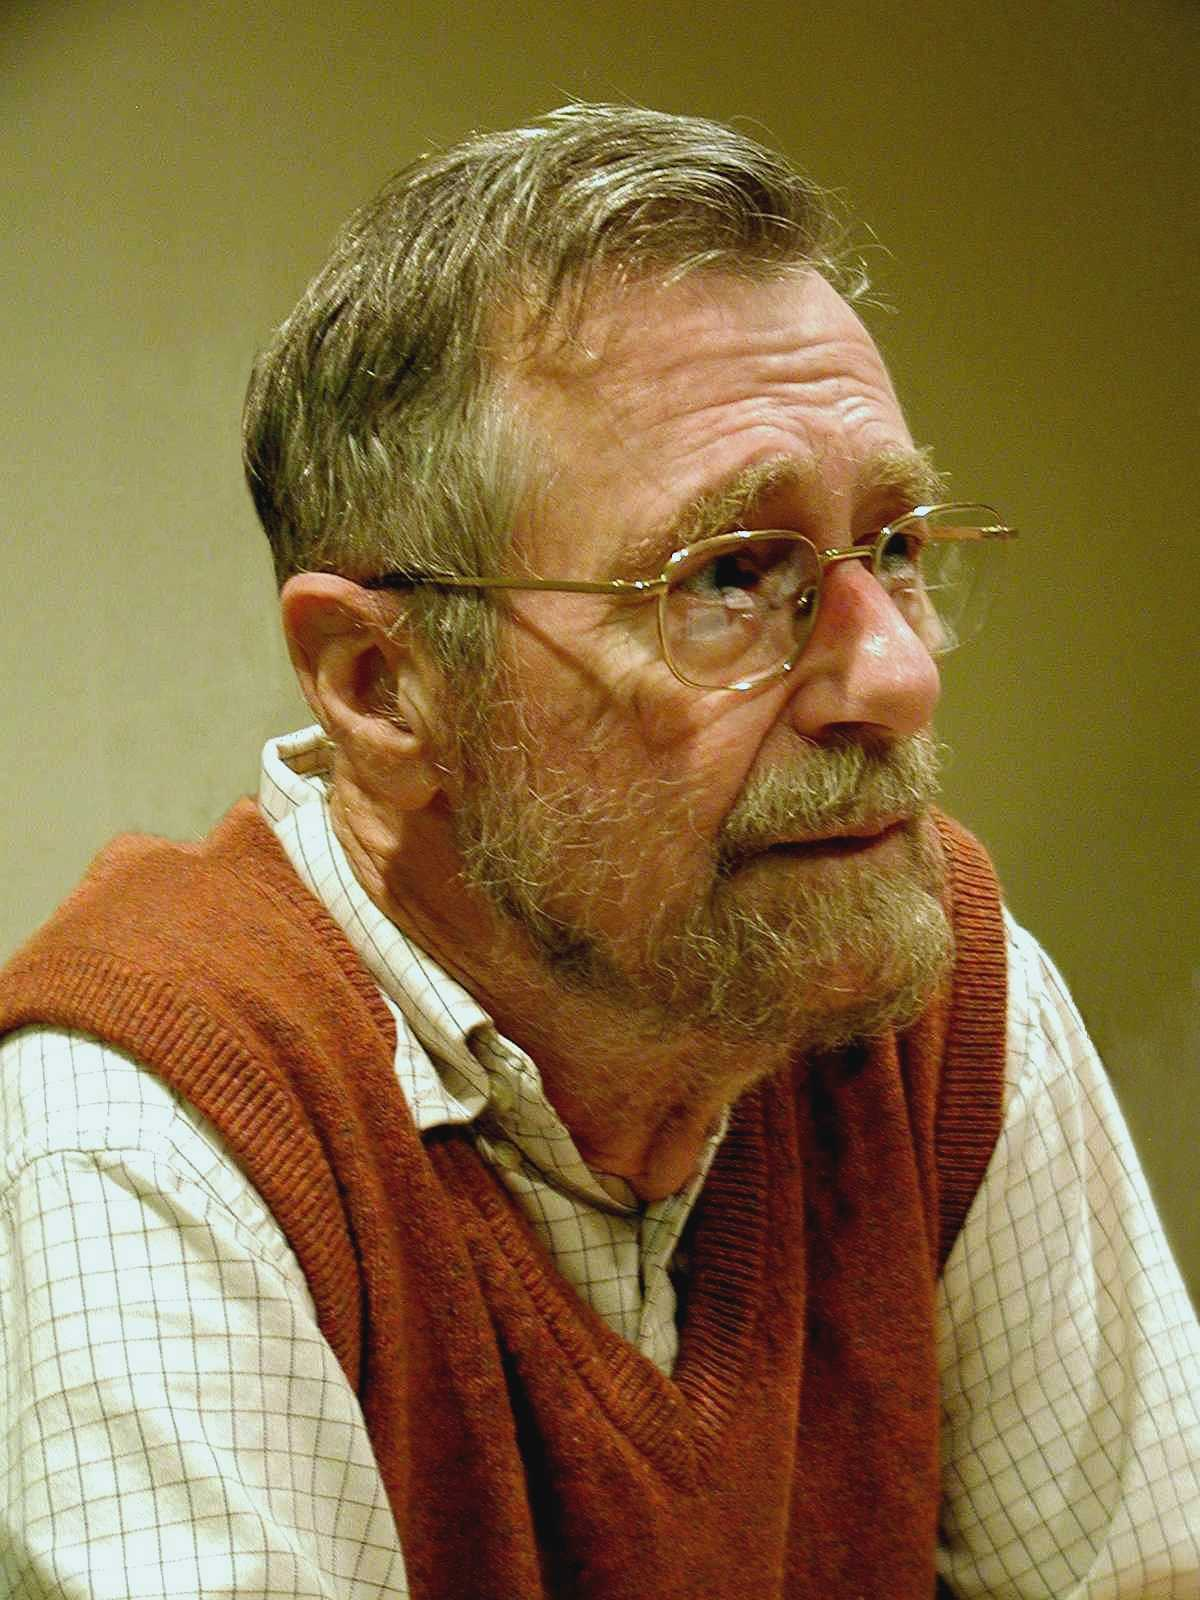
\includegraphics[height=1.15in]{images/dijkstra.jpg}\par
\medskip
{\small\itshape ``programming is as hard or as easy as proving''\par}
\smallskip
{\small Edsger W. Dijkstra\par}
{\scriptsize\href{https://www.cs.utexas.edu/~EWD/transcriptions/EWD12xx/EWD1243a.html}{\emph{The next fifty years} (excerpt)}\par}
\smallskip
{\scriptsize Photo: \copyright\ 2002 Hamilton Richards;\\
\href{https://www.cs.utexas.edu/~EWD/}{E. W. Dijkstra Archive, UT Austin}.\par}
\end{minipage}\hfill
\begin{minipage}[t]{0.46\textwidth}
\centering
\vspace{0pt}
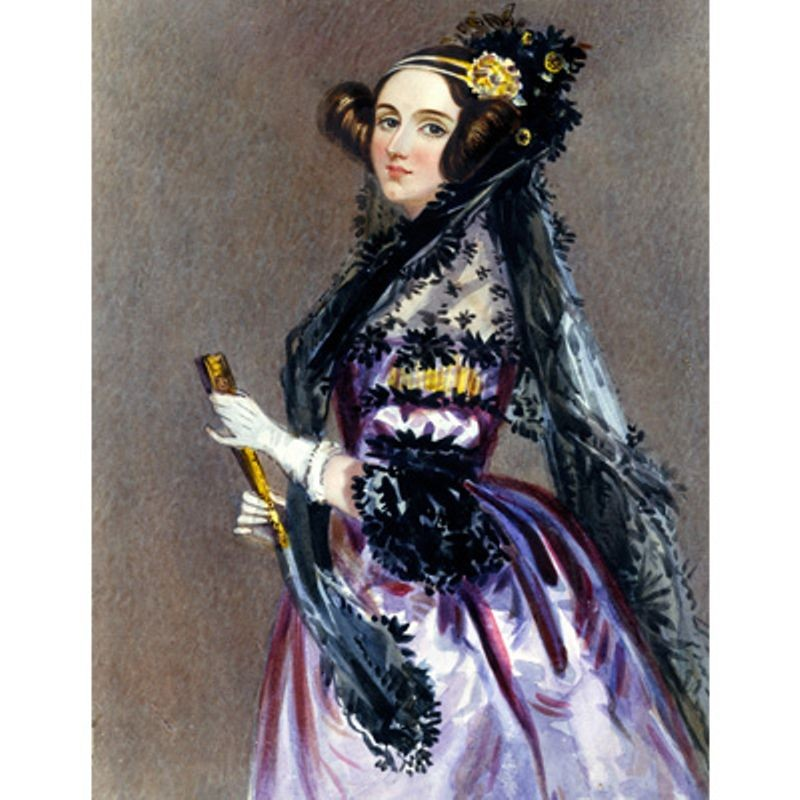
\includegraphics[height=1.15in]{images/lovelace.jpg}\par
\medskip
{\small\itshape ``The Analytical Engine weaves algebraic patterns just as the
Jacquard loom weaves flowers and leaves.''\par}
\smallskip
{\small Ada Lovelace, 1843\par}
{\scriptsize\href{https://www.computerhistory.org/babbage/adalovelace/}{As reproduced by the Computer History Museum}\par}
\smallskip
{\scriptsize Portrait, c. 1838: Science Museum;\\
via the Computer History Museum.\par}
\end{minipage}
\end{center}
\medskip

In the chapter on proofs, induction allowed us to establish infinitely many
claims using a base case and an inductive step. A closely related idea lets us
\emph{compute}: give the answer for a base case, and describe how to obtain a
new answer from answers to smaller problems. We have already done this when
we defined addition using the successor function. We now make that idea into
a model of computation.

\section{Why do we need a model of computation?}

An algorithm is a finite, unambiguous description of a procedure for obtaining
an answer from an input. For an algorithm that solves a problem on a stated
domain, the procedure must terminate and give the right answer on every input
in that domain. A description such as ``find the answer'' is not enough: we
must say what operations are available and how to combine them.

A model of computation supplies these rules. It separates the mathematical
procedure from the machine, programming language, or representation used to
carry it out. It also makes three different questions precise: what answer
is required, whether a procedure computes that answer, and how much work the
procedure takes. Two procedures can compute the same function with very
different amounts of work.

Our starting point is a function $f:\N\rightarrow\N$, where, as earlier,
$\N=\{0,1,2,\ldots\}$. An input is a natural number and a terminating
computation produces a natural number. We freely use functions of several
arguments, such as $\operatorname{add}:\N^2\rightarrow\N$. Using several arguments makes the notation easier to read. Pairs can be encoded as
single natural numbers; for example,
\[
\langle a,b\rangle=\frac{(a+b)(a+b+1)}{2}+b.
\]
This lists pairs by successive diagonals of $\N^2$. Its encoding and decoding
are effective finite procedures. Repeating the construction encodes tuples.
Finite strings, lists, and other finite data can likewise be represented by
natural numbers. This explains why numerical functions are a useful starting
point even when the eventual application concerns words or pictures.\footnote{
Ada Lovelace met Charles Babbage in 1833, when she was seventeen, and saw
him demonstrate a working section of his calculating engine. In her 1843
notes she went beyond arithmetic to envisage operations on other kinds of
symbols, even the composition of music. See the
\href{https://www.computerhistory.org/babbage/adalovelace/}{Computer History
Museum's account}.}

\section{Functions defined by induction}

Recall the successor function $S(n)=n+1$. We may start with zero, successor,
and functions that select an argument, and build new functions by
\emph{composition} and \emph{recursion}. Composition means using the output
of one function as the input of another: $h(n)=g(f(n))$.
A basic recursion scheme is
\[
f(\mathbf{x},m)=\begin{cases}
g(\mathbf{x}),&\text{if }m=0,\\
h(\mathbf{x},n,f(\mathbf{x},n)),&\text{otherwise}.
\end{cases}
\]
Here $\mathbf{x}$ denotes a tuple of additional arguments, and $g$ and $h$
are functions already constructed. In the otherwise branch, $n$ denotes
the unique predecessor of $m$, so $m=S(n)$; this branch is used only when
$m>0$. The recursive call decreases the last argument by one. These rules
determine a unique value on every input, provided the computations of $g$
and $h$ always finish on the inputs used.
This scheme is called \emph{primitive recursion}.

\subsection{Addition and multiplication}

Write $\operatorname{pred}(b)$ for the predecessor of a positive $b$, so
$\operatorname{pred}(S(n))=n$. It is used only in the nonzero branch.
To compute $a+b$, begin with $a+0=a$. If we can compute $a+n$, applying
successor gives $a+S(n)$. This proof pattern gives the algorithm
\[
\operatorname{add}(a,b)=\begin{cases}
a,&\text{if }b=0,\\
S(\operatorname{add}(a,\operatorname{pred}(b))),&\text{otherwise}.
\end{cases}
\]
\textbf{Correctness, by induction on $b$.}
\emph{Basis:} $\operatorname{add}(a,0)=a=a+0$ for every $a$.
\emph{Induction hypothesis:} for an arbitrary integer $n\geq0$ and every $a\in\N$,
$\operatorname{add}(a,n)=a+n$.
\emph{Inductive step:}
\[
\operatorname{add}(a,S(n))=S(\operatorname{add}(a,n))
=S(a+n)=a+S(n).
\]
The call decreases $b$ to its predecessor, so it also terminates.

For multiplication, the base product is zero. If we can compute $an$, one
more addition of $a$ gives $aS(n)$. Thus
\[
\operatorname{mul}(a,b)=\begin{cases}
0,&\text{if }b=0,\\
\operatorname{add}(\operatorname{mul}(a,\operatorname{pred}(b)),a),&\text{otherwise}.
\end{cases}
\]
\textbf{Correctness, by induction on $b$.}
\emph{Basis:} $\operatorname{mul}(a,0)=0=a\cdot0$.
\emph{Induction hypothesis:} for an arbitrary integer $n\geq0$,
$\operatorname{mul}(a,n)=an$ for every $a\in\N$.
\emph{Inductive step:} using the already established correctness of addition,
\[
\operatorname{mul}(a,S(n))
=\operatorname{add}(\operatorname{mul}(a,n),a)=an+a=aS(n).
\]
Again, the second argument decreases to zero. For example,
$\operatorname{mul}(4,3)$ computes $4+4+4$ through three additions to an
initial zero.

\paragraph{A notational simplification.}
From here onwards, we write $n+1$ instead of $S(n)$, and $n-1$ for the
predecessor when $n>0$. We also use ordinary addition and multiplication
symbols for the functions just constructed. These symbols abbreviate the computations we have just defined.

\subsection{Conditions, specifications, and algorithms}

Our specification language also includes \emph{if--then--else}. For example,
\[
K(x)=\begin{cases}
u(x),&\text{if }C(x),\\
v(x),&\text{otherwise}.
\end{cases}
\]
First evaluate the condition $C(x)$. If it is true, compute $u(x)$;
otherwise compute $v(x)$. Only the selected branch is evaluated. With more
than two cases, test the conditions in order and use the first that holds;
``otherwise'' covers the remaining inputs. For this to be an algorithm,
the test itself must have a definite computational procedure. The curly
braces alone do not make a mathematical specification executable.

For example, consider the following specification:
\[
\operatorname{sqrt}(n)=\begin{cases}
m,&\text{if some }m\in\N\text{ satisfies }m^2=n,\\
0,&\text{otherwise}.
\end{cases}
\]
The natural-number root, when it exists, is unique. This is a valid
specification: return the exact root for a perfect square and zero otherwise.
It also returns zero for $n=0$; zero is therefore not a distinct failure code.
But the first condition neither says how to find $m$ nor how to establish
that none exists. This description states the required answer without yet
providing a method of computing it.

A procedure can start with a candidate $m=0$ and test successive candidates:
\[
R(n,m)=\begin{cases}
m,&\text{if }m^2=n,\\
0,&\text{if }m^2>n,\\
R(n,m+1),&\text{otherwise}.
\end{cases}
\]
Evaluate $R(n,0)$. Each test is computable using multiplication and comparison.
Candidates smaller than $m$ have already been checked; once $m^2>n$, no
larger candidate can succeed. The search stops no later than $m=n+1$.
Thus it returns exactly the value specified above. For example,
$R(9,0)=R(9,1)=R(9,2)=R(9,3)=3$, whereas the search for $8$ stops at
$m=3$ and returns zero. The distinction is between a condition describing
an answer and instructions that actually find it.

We read our algorithmic equations as evaluation rules from left to right.
An equation such as $f(n)=f(n)$, by itself, gives no procedure for finding a
value. Neither a familiar function name nor mathematically valid notation
supplies the missing computational steps.

\paragraph{An algorithm can be read from a proof.}
The examples suggest a method of construction. Rather than guess a sequence
of steps, start with what is to be computed. Find a base case that can
be solved directly. Then assume that a smaller instance can be solved, and
show how its answer gives the answer to the current instance. The algorithm
is a \emph{computational rendering of this inductive proof}: the base case
becomes a stopping rule, the induction hypothesis becomes a recursive call,
and the inductive step becomes the computation using its result. Finding a
useful induction may require ingenuity, but the proof guides the construction.
\footnote{Dijkstra once illustrated the limits of exhaustive testing with
his university's multiplication hardware: at the quoted speed, trying every
possible pair of inputs would take roughly 30,000 years. His point was that
understanding why a procedure works can cover cases that we will never have
time to test individually. See
\href{https://www.cs.utexas.edu/~EWD/transcriptions/EWD03xx/EWD303.html}{EWD303,
``On the reliability of programs''}.}

A recursive call need not decrease an argument by exactly one. It may
decrease some other natural-number measure. The Well-Ordering Principle
rules out an infinite descent; induction on that measure proves correctness.
In the examples below, we make both the measure and the proof explicit.

\subsection{Quotient and remainder}
\label{sec:alg-division}

For $b>0$, the division theorem gives $a=bq+r$, with $0\leq r<b$.
We use \emph{induction on the quotient $q$} to construct the algorithms.
When $q=0$, $a<b$, so the quotient is zero and the remainder is $a$.
If $a=b(q+1)+r$, subtracting $b$ leaves $bq+r$: solve this smaller-quotient
problem, add one to its quotient, and keep its remainder. This gives
\[
\operatorname{div}(a,b)=\begin{cases}
0,&\text{if }a<b,\\
\operatorname{div}(a-b,b)+1,&\text{otherwise},
\end{cases}
\]
\[
\operatorname{mod}(a,b)=\begin{cases}
a,&\text{if }a<b,\\
\operatorname{mod}(a-b,b),&\text{otherwise}.
\end{cases}
\]
Subtraction and comparison are the natural-number operations introduced
earlier. Here $a-b$ is used only when $a\geq b$.

\textbf{Correctness, by induction on $q$.}
The precise claim is: for every $q\geq0$, every $b>0$, and every
$0\leq r<b$,
\[
\operatorname{div}(bq+r,b)=q,\qquad
\operatorname{mod}(bq+r,b)=r.
\]
\emph{Basis:} when $q=0$, the first argument is $r<b$, so the two base
branches return $0$ and $r$.
\emph{Induction hypothesis:} for an arbitrary integer $q\geq0$, both claims
hold for all $b>0$ and $0\leq r<b$.
\emph{Inductive step:} for $a=b(q+1)+r$, we have $a\geq b$ and $a-b=bq+r$.
Consequently,
\[
\begin{aligned}
\operatorname{div}(a,b)&=\operatorname{div}(bq+r,b)+1=q+1,\\
\operatorname{mod}(a,b)&=\operatorname{mod}(bq+r,b)=r.
\end{aligned}
\]
Each call reduces the quotient by one, so after $q$ calls the base case is
reached. The algorithm need not \emph{know} $q$ in advance: $q$ is the
measure used in its proof, and $a<b$ detects the stopping case.
For example,
\[
\begin{aligned}
\operatorname{div}(17,5)&=\operatorname{div}(12,5)+1
=(\operatorname{div}(7,5)+1)+1=3,\\
\operatorname{mod}(17,5)&=\operatorname{mod}(12,5)
=\operatorname{mod}(7,5)=\operatorname{mod}(2,5)=2.
\end{aligned}
\]
Division by zero is excluded from the domain.

\subsection{Powers and factorials}
\label{sec:alg-powers-factorials}

For $x,n\in\N$, the identities $x^0=1$ and $x^n=x^{n-1}x$ suggest
\[
\operatorname{pow}(x,n)=\begin{cases}
1,&\text{if }n=0,\\
\operatorname{pow}(x,n-1)\cdot x,&\text{otherwise}.
\end{cases}
\]
\textbf{Correctness, by induction on $n$.}
\emph{Basis:} $\operatorname{pow}(x,0)=1=x^0$.
\emph{Induction hypothesis:} for an arbitrary integer $k\geq0$,
$\operatorname{pow}(x,k)=x^k$ for every $x\in\N$.
\emph{Inductive step:}
$\operatorname{pow}(x,k+1)=\operatorname{pow}(x,k)x=x^kx=x^{k+1}$.
We adopt $0^0=1$ in this discrete definition, consistent with the empty
product. The exponent decreases to zero.

Similarly, $0!=1$ and $n!=n(n-1)!$ give
\[
\operatorname{fact}(n)=\begin{cases}
1,&\text{if }n=0,\\
n\cdot\operatorname{fact}(n-1),&\text{otherwise}.
\end{cases}
\]
\textbf{Correctness, by induction on $n$.}
\emph{Basis:} $\operatorname{fact}(0)=1=0!$.
\emph{Induction hypothesis:} for an arbitrary integer $k\geq0$,
$\operatorname{fact}(k)=k!$.
\emph{Inductive step:}
\[
\operatorname{fact}(k+1)=(k+1)\operatorname{fact}(k)=(k+1)k!=(k+1)!.
\]
The argument decreases to zero, proving termination. In each example, the
same induction both suggests the algorithm and establishes its correctness.

\subsection{Unfolding recursion: work that waits}
\label{sec:alg-deferred}

Let us follow the factorial algorithm exactly, at the level where
multiplication is available. Each recursive call leaves a multiplication
waiting for its answer:
\[
\begin{aligned}
\operatorname{fact}(5)
 &=5\cdot\operatorname{fact}(4)\\
 &=5\cdot(4\cdot\operatorname{fact}(3))\\
 &=5\cdot(4\cdot(3\cdot\operatorname{fact}(2)))\\
 &=5\cdot(4\cdot(3\cdot(2\cdot\operatorname{fact}(1))))\\
 &=5\cdot(4\cdot(3\cdot(2\cdot(1\cdot\operatorname{fact}(0)))))\\
 &=5\cdot(4\cdot(3\cdot(2\cdot(1\cdot1))))\\
 &=5\cdot(4\cdot(3\cdot(2\cdot1)))\\
 &=5\cdot(4\cdot(3\cdot2))\\
 &=5\cdot(4\cdot6)\\
 &=5\cdot24\\
 &=120.
\end{aligned}
\]
The expression first grows as the calls descend to zero. No multiplication
can yet be completed under these evaluation rules: the inner answer is not
available. After the base value $1$ is obtained, the expression shrinks as
the pending multiplications are performed. These are \emph{deferred
computations}. A direct evaluator remembers the unfinished calls in a
\emph{stack}.

Contrast this with computing the successive products $1,5,20,60,120,120$
as we count down from $5$ to $0$. Here every multiplication can be completed
immediately, and its result carried forward. In
Section~\ref{sec:alg-iteration} we will derive the tail-recursive algorithm
for this second process and trace the same input. Both function definitions
are recursive; only the first process accumulates deferred multiplications.

\subsection{Summing the values of a function}
\label{sec:alg-sum}

Suppose a procedure for computing $f(i)\in\N$ is already available and
finishes for every argument used. We want to compute
$\sum_{i=a}^{b}f(i)$ for $a,b\in\N$, taking an empty sum ($a>b$) as zero.
The empty interval is the base case. For a nonempty interval, the first term
plus the sum of the remaining terms gives the required answer:
\[
\operatorname{Sum}_f(a,b)=\begin{cases}
0,&\text{if }a>b,\\
f(a)+\operatorname{Sum}_f(a+1,b),&\text{otherwise}.
\end{cases}
\]
The subscript $f$ means that we use a fixed, already available function;
choosing another $f$ gives another summation procedure. For $f(i)=i^2$,
\[
\operatorname{Sum}_f(2,4)=4+(9+(16+0))=29.
\]
The additions are deferred until the recursive answers are available.

\textbf{Correctness, by induction on the number $\ell$ of terms.}
Here $\ell=0$ if $a>b$, and $\ell=b-a+1$ otherwise.
\emph{Basis:} an empty interval returns $0$, the empty sum.
\emph{Induction hypothesis:} for an arbitrary integer $k\geq0$, the
procedure returns the correct sum for \emph{every} interval of $k$ terms.
\emph{Inductive step:} an interval $[a,b]$ of $k+1$ terms has $k$ terms
remaining in $[a+1,b]$. Therefore
\[
\operatorname{Sum}_f(a,b)
=f(a)+\operatorname{Sum}_f(a+1,b)
=f(a)+\sum_{i=a+1}^{b}f(i)=\sum_{i=a}^{b}f(i).
\]
Each call removes one term, so the computation terminates. Notice that the
first argument increases: it is the \emph{number of remaining terms} that
decreases. Taking $f(i)=i$, $i^2$, or $1$ gives sums of integers, sums of
squares, or a count of terms using the same proof and algorithm.

\section{How much work? Complexity and Big O}

Correctness does not tell us whether a computation is practical.
\emph{Time complexity} counts work as the input grows; \emph{space
complexity} measures the storage needed. We begin by counting the main
operations: additions in summation, multiplications in factorial and powers,
and remainder computations in Euclid's algorithm.\footnote{These counts use
whole-number operations as units of work. They need not equal counts of
successor operations or individual bit operations. For example, a remainder
computed by repeated subtraction may require many elementary steps. A more
detailed analysis would expand the operations being counted.}\footnote{A
number's value and the length of its representation are different measures.
In binary, $n\geq1$ has $L=\lfloor\log_2 n\rfloor+1$ bits. A procedure
using $n$ steps can therefore take order $2^L$ steps in the input length.
Large-number arithmetic also costs more than small-number arithmetic.
We set these questions of bit complexity aside in this first discussion.}

\subsection{Recurrences count the work}

A \emph{time-complexity recurrence} expresses the work on an input in terms
of the work of its recursive calls, plus the work done outside those calls.
It has a base case, just like the algorithm. This is an important tool for
estimating steps: identify the calls, count the extra work, then unfold the
recurrence or bound its solution by induction. Count every recursive call;
two calls to the same smaller problem are still two computations unless
the result is explicitly computed once and reused.

For factorial, let $T(n)$ count multiplications. Reading the definition gives
\[
T(n)=\begin{cases}
0,&\text{if }n=0,\\
1+T(n-1),&\text{otherwise}.
\end{cases}
\]
Unfolding gives $T(n)=1+T(n-1)=2+T(n-2)=\cdots=n+T(0)=n$.
There are also $n+1$ factorial calls, and at most $n$ pending multiplications.
This measures the work of this algorithm, not a lower bound for every
possible factorial algorithm.

For summation, counting one addition per term gives
\[
A(\ell)=\begin{cases}
0,&\text{if }\ell=0,\\
A(\ell-1)+1,&\text{otherwise},
\end{cases}
\qquad\text{so }A(\ell)=\ell.
\]
There are also $\ell$ evaluations of $f$.\footnote{If evaluating $f(i)$
costs $C_f(i)$ steps, the full count includes $\sum_{i=a}^{b}C_f(i)$ as
well as additions and bookkeeping. Our addition count isolates the work
of the summation procedure itself.}

For successor-based addition, exactly $b$ successor operations are performed,
so the work grows linearly with $b$. Multiplication makes $b$ additions,
each applying successor $a$ times, for a total of $ab$ successor operations.
These simple counts already distinguish linear growth from growth in the
product of two inputs.\footnote{Including tests and call bookkeeping adds
work proportional to the number of calls. Under a constant cost for each
such step, addition is bounded by a constant times $b+1$, and multiplication
by a constant times $ab+b+1$. The extra terms account for zero inputs too.}

\begin{definition}[Big O]
For nonnegative functions $T$ and $g$, we write $T(n)=O(g(n))$ if there are
constants $C>0$ and $n_0$ such that
\[
T(n)\leq Cg(n)\qquad\text{for all }n\geq n_0.
\]
\end{definition}
Thus $3n+7=O(n)$: for $n\geq1$, $3n+7\leq10n$. Constant factors and
lower-order terms do not affect this upper bound. Big O need not be tight:
$3n+7$ is also $O(n^2)$, although the linear bound tells us more. Typical
orders of growth are $O(1)$, $O(\log n)$, $O(n)$, $O(n\log n)$, $O(n^2)$, and $O(2^n)$.
Big O itself does not mean ``worst case''; we first choose whether $T$
measures worst-case, average, or some particular execution cost.

\subsection{Seeing the difference in growth rates}

Figure~\ref{fig:alg-growth} plots representative functions for the five
orders of growth. The curves are $\log_2 n$, $n$, $n\log_2 n$, $n^2$,
and $2^n$ themselves: Big O denotes a class of upper bounds, not one
particular curve. Constant factors are taken as one for comparison.

\begin{figure}[htbp]
\centering
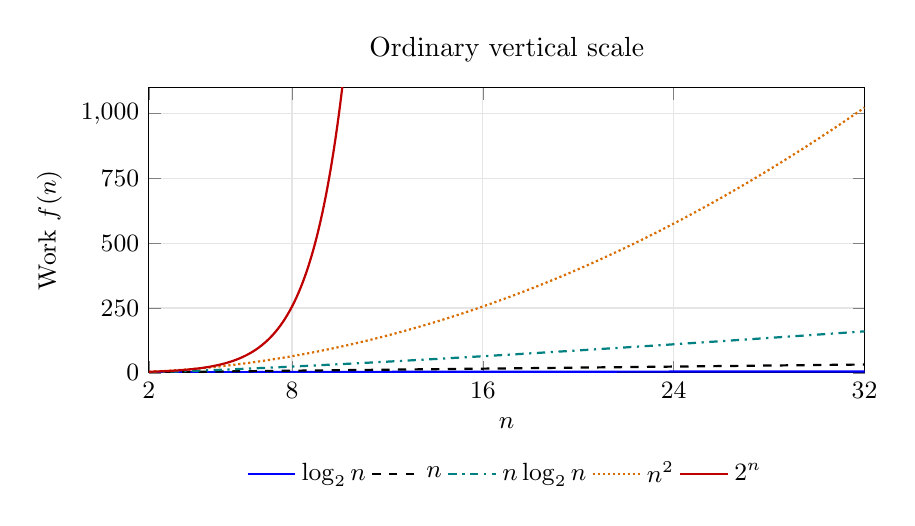
\begin{tikzpicture}
\begin{axis}[
width=0.88\textwidth,height=5.2cm,
xmin=2,xmax=32,ymin=0,ymax=1100,
xlabel={$n$},ylabel={Work $f(n)$},
title={Ordinary vertical scale},
xtick={2,8,16,24,32},ytick={0,250,500,750,1000},
grid=major,grid style={gray!20},
tick label style={font=\small},label style={font=\small},
legend style={font=\small,at={(0.5,-0.27)},anchor=north,draw=none},
legend columns=5]
\addplot[blue,thick,domain=2:32,samples=100] {ln(x)/ln(2)};
\addlegendentry{$\log_2 n$}
\addplot[black,thick,dashed,domain=2:32] {x};
\addlegendentry{$n$}
\addplot[teal,thick,dashdotted,domain=2:32,samples=100] {x*ln(x)/ln(2)};
\addlegendentry{$n\log_2 n$}
\addplot[orange!85!black,thick,densely dotted,domain=2:32,samples=100] {x*x};
\addlegendentry{$n^2$}
\addplot[red!75!black,thick,domain=2:11,samples=100] {2^x};
\addlegendentry{$2^n$}
\end{axis}
\end{tikzpicture}

\medskip
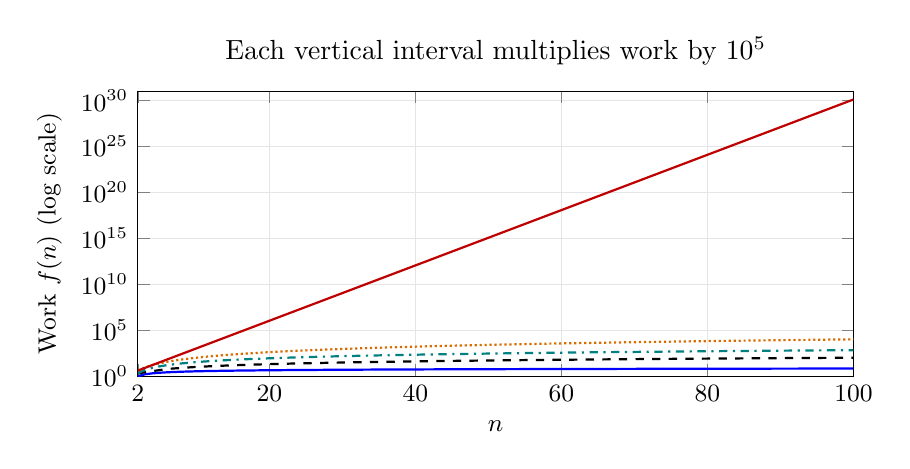
\begin{tikzpicture}
\begin{semilogyaxis}[
width=0.88\textwidth,height=5.2cm,
xmin=2,xmax=100,ymin=1,ymax=1e31,
xlabel={$n$},ylabel={Work $f(n)$ (log scale)},
title={Each vertical interval multiplies work by $10^5$},
xtick={2,20,40,60,80,100},
ytick={1,1e5,1e10,1e15,1e20,1e25,1e30},
grid=major,grid style={gray!20},
tick label style={font=\small},label style={font=\small}]
\addplot[blue,thick,domain=2:100,samples=100] {ln(x)/ln(2)};
\addplot[black,thick,dashed,domain=2:100] {x};
\addplot[teal,thick,dashdotted,domain=2:100,samples=100] {x*ln(x)/ln(2)};
\addplot[orange!85!black,thick,densely dotted,domain=2:100,samples=100] {x*x};
\addplot[red!75!black,thick,domain=2:100,samples=100] {2^x};
\end{semilogyaxis}
\end{tikzpicture}
\caption{Five growth rates on two scales; the same styles identify curves
in both panels. In the upper panel, $2^n$ leaves the displayed range just
after $n=10$. The logarithmic scale below keeps it visible up to $n=100$;
its straight appearance there represents exponential growth.}
\label{fig:alg-growth}
\end{figure}

Doubling $n$ adds one to $\log_2 n$, doubles $n$, changes $n\log_2 n$
by a factor $2(1+1/\log_2 n)$, and quadruples $n^2$. For $2^n$, doubling
$n$ \emph{squares the amount of work}. Even increasing $n$ by just one
doubles it. These statements concern the displayed functions, not arbitrary
algorithms known only to satisfy the corresponding Big O upper bounds.

\paragraph{How bad is exponential growth?}
Suppose an algorithm actually performs $2^n$ steps, and imagine a machine
performing a billion ($10^9$) of those steps each second. Then:
\begin{center}
\begin{tabular}{r r l}
\hline
$n$ & Steps $2^n$ (approximately) & Time (approximately)\\
\hline
10 & $1.02\times10^3$ & $1.02$ microseconds\\
30 & $1.07\times10^9$ & $1.07$ seconds\\
50 & $1.13\times10^{15}$ & $13$ days\\
100 & $1.27\times10^{30}$ & $4.02\times10^{13}$ years\\
\hline
\end{tabular}
\end{center}
At $n=100$, the other four representative counts are only about $6.64$,
$100$, $664$, and $10{,}000$. A machine a thousand times faster buys the
exponential algorithm only $\log_2 1000\approx10$ additional units of input
in the same time budget. Better hardware changes a constant factor; a
better algorithm may change the growth rate. Exponential algorithms can
still be useful for small inputs, but scale very poorly. An $O(2^n)$ upper
bound alone does not establish exponential behaviour; the example assumes
an actual $2^n$ step count.

\subsection{A faster way to compute powers}
\label{sec:alg-fast-power}

The power algorithm removes one factor at a time. Can we make a bigger
reduction? If we know $x^k$, one squaring gives $x^{2k}$; one further
multiplication by $x$ gives $x^{2k+1}$. Define the helper
\[
\operatorname{sqr}(y)=y\cdot y.
\]
Then use the parity of the exponent to choose the appropriate rule:
\[
E(x,n)=\begin{cases}
1,&\text{if }n=0,\\
\operatorname{sqr}(E(x,\operatorname{div}(n,2))),&\text{if }n\text{ is even},\\
x\cdot\operatorname{sqr}(E(x,\operatorname{div}(n,2))),&\text{otherwise}.
\end{cases}
\]
Only one branch is used. In that branch the argument of $\operatorname{sqr}$
is evaluated once; the helper then multiplies the resulting number by itself.
Thus there is just one recursive call at each level.

\textbf{Correctness, by strong induction on the exponent $n$.}
\emph{Basis:} $E(x,0)=1=x^0$ for every $x\in\N$.
\emph{Induction hypothesis:} for an arbitrary integer $n\geq1$, assume
$E(x,j)=x^j$ for every integer $0\leq j<n$ and every $x\in\N$.
\emph{Inductive step:} put $k=\operatorname{div}(n,2)$, so $0\leq k<n$.
If $n=2k$, the algorithm returns $(x^k)^2=x^n$ by the hypothesis.
If $n=2k+1$, it returns $x(x^k)^2=x^n$. In both cases the recursive
exponent is smaller, so the computation also terminates.

\paragraph{Deriving the logarithmic bound.}
Let $M(n)$ be the number of multiplications made by this fast-power algorithm.
Its exact recurrence is
\[
M(n)=\begin{cases}
0,&\text{if }n=0,\\
M(\lfloor n/2\rfloor)+1,&\text{if }n>0\text{ is even},\\
M(\lfloor n/2\rfloor)+2,&\text{otherwise}.
\end{cases}
\]
There is one recursive call; an even exponent adds one multiplication,
and an odd exponent adds two. For $n\geq1$, after
$L=\lfloor\log_2 n\rfloor+1$ halvings the exponent is zero. Hence
\[
L\leq M(n)\leq2L,
\qquad M(n)=O(\log{n}).
\]
Equivalently, unfold the upper-bound recurrence
$M(n)\leq M(\lfloor n/2\rfloor)+2$ for $L$ levels.
For $n=16$, the exponents are $16,8,4,2,1,0$, and the count is
$1+1+1+1+2=6$, compared with $16$ multiplications for ordinary power.

The helper $\operatorname{sqr}$ matters. Replacing it by two separate calls
$E(x,\operatorname{div}(n,2))\cdot E(x,\operatorname{div}(n,2))$ would repeat
the smaller computation. For even $n$, the new multiplication count would
satisfy $D(n)=2D(n/2)+1$. Unfolding this recurrence for $n=2^k$ gives
$D(2^k)=3\cdot2^k-1$, since $D(1)=2$: the count is now linear in $n$.
Halving the problem helps only if we avoid doing the same work twice.
\footnote{The logarithmic bound counts multiplications. It treats the
halving and parity tests as auxiliary operations; implementing division by
repeated subtraction would add further work. The sizes of the multiplied
numbers matter in a bit-operation analysis.}

\subsection{Euclid's algorithm: correctness and efficiency}
\label{sec:alg-euclid}

For $a,b\in\N$ not both zero, the greatest common divisor is the largest
positive integer dividing both. Euclid's algorithm gives a particularly
clear example of a proof guiding an efficient computation.\footnote{In
\href{https://mathcs.clarku.edu/~djoyce/elements/bookVII/propVII2.html}{Book VII,
Proposition 2 of the \emph{Elements}}, Euclid describes the reduction by
continually subtracting the smaller number from the larger. Computing a
remainder packages several such subtractions into one step. The notation
has changed, but the common-divisor argument is the same.} Its key is the
following claim.

\textbf{Claim.} If $a=bq+r$, $b>0$, and $0\leq r<b$, then
$\gcd(a,b)=\gcd(b,r)$.
\emph{Proof:} let $d=\gcd(a,b)$. Since $d$ divides both $a$ and $b$, it
divides $r=a-bq$, so it is a common divisor of $b,r$. Conversely, any
positive common divisor $c$ of $b,r$ divides $bq+r=a$, so it is a common
divisor of $a,b$ and hence $c\leq d$. Thus $d$ is the greatest common
divisor of $b,r$. This includes $r=0$.

The claim reduces the second argument from $b$ to $r<b$. Assuming we can
solve all such smaller cases, we obtain the algorithm
\[
G(a,b)=\begin{cases}
a,&\text{if }b=0,\\
G(b,\operatorname{mod}(a,b)),&\text{otherwise}.
\end{cases}
\]
\textbf{Correctness, by strong induction on $b$.}
We prove $G(a,b)=\gcd(a,b)$ for every $b\geq0$ and \emph{every} $a>0$.
\emph{Basis:} $G(a,0)=a=\gcd(a,0)$.
\emph{Induction hypothesis:} for an arbitrary integer $k\geq0$,
assume that for all integers $0\leq j\leq k$ and all $u>0$,
$G(u,j)=\gcd(u,j)$.
\emph{Inductive step:} let $b=k+1$ and $r=\operatorname{mod}(a,b)$.
Since $0\leq r<b$ and $b>0$,
\[
G(a,b)=G(b,r)=\gcd(b,r)=\gcd(a,b).
\]
The middle equality uses the induction hypothesis, and the last uses the
claim. Quantifying over \emph{every} first argument is essential: the
recursive call changes it from $a$ to $b$. The decreasing second argument
also proves termination.

For completeness, if $a=0<b$, the algorithm returns $G(b,0)=b$, as required.
We may set $G(0,0)=0$ by convention to obtain a numerical function defined on every pair;
this does not assert that zero has a greatest positive divisor.
For example,
\[
G(48,18)=G(18,12)=G(12,6)=G(6,0)=6.
\]
The following chapter on primes and gcd develops the number-theoretic
consequences further.

\paragraph{Why logarithmically many steps?}

Let $C(a,b)$ count remainder computations. Directly from the algorithm,
\[
C(a,b)=\begin{cases}
0,&\text{if }b=0,\\
1+C(b,\operatorname{mod}(a,b)),&\text{otherwise}.
\end{cases}
\]
Merely observing that the second argument decreases proves termination,
but gives only a crude linear bound. We need to show that it shrinks quickly.
Put $r=\operatorname{mod}(a,b)$, so $0\leq r<b$. If $r=0$, we stop after
one step. If $0<r\leq b/2$, the new second argument is already at most half
of $b$. Otherwise $b/2<r<b$, so the next remainder is
\[
\operatorname{mod}(b,r)=b-r<b/2,
\]
because $b$ contains exactly one copy of $r$. Thus within at most two
remainder steps, either the computation stops or its second argument at
least halves.

After at most $2\lceil\log_2 b\rceil$ steps, a starting $b\geq1$ has
therefore either reached zero or become at most $1$; one further step then
finishes. Hence
\[
C(a,b)\leq2\lceil\log_2 b\rceil+1\quad(b\geq1).
\]
This shows that the algorithm requires $O(\log b)$  steps. It requires no assumption that $a\geq b$.\footnote{The
bound counts remainder computations. It does not count the subtractions
or bit operations used to implement each remainder.}

\section{Iteration through tail recursion}
\label{sec:alg-iteration}

Return to factorial. To avoid deferred multiplications, let $p$ record the
product already computed and $k$ count the factors still to be processed.
We want $p=n!$ when $k=0$. A useful relation to maintain throughout is
\[
0\leq k\leq n,\qquad p\cdot k!=n!.
\]
Initially this holds with $(k,p)=(n,1)$. If $k>0$, replacing $(k,p)$ by
$(k-1,pk)$ preserves the relation, since $(pk)(k-1)!=pk!$.
This reasoning \emph{derives} the algorithm
\[
F(k,p)=\begin{cases}
p,&\text{if }k=0,\\
F(k-1,p\cdot k),&\text{otherwise}.
\end{cases}
\]
To compute $n!$, evaluate $F(n,1)$. Its evaluation for $n=5$ is
\[
\begin{aligned}
F(5,1)&=F(4,5)\\
      &=F(3,20)\\
      &=F(2,60)\\
      &=F(1,120)\\
      &=F(0,120)\\
      &=120.
\end{aligned}
\]
At each transition the multiplication is carried out \emph{before} the next
call. Compare the two factorial computations:
\begin{center}
\begin{tabular}{p{0.43\textwidth} p{0.43\textwidth}}
\hline
\textbf{Deferred computation} & \textbf{Direct accumulation}\\
\hline
$5\cdot\operatorname{fact}(4)$ waits for the inner answer.
& $F(5,1)\longrightarrow F(4,5)$ carries a completed product.\\
Pending multiplications accumulate, then are performed on return.
& Completed products are carried forward in $p$.\\
The evaluator remembers unfinished work.
& The current state $(k,p)$ contains all the information needed.\\
\hline
\end{tabular}
\end{center}

In $F$, nothing remains to be done with the result of the recursive call.
Such a call is in \emph{tail position}; a function whose recursive calls
all have this form is \emph{tail recursive}. A recursively written function
can therefore generate an \emph{iterative process}: repeatedly replace a
current state by a next state, without accumulating unfinished calls.
In general,
\[
I(s)=\begin{cases}
\operatorname{answer}(s),&\text{if }\operatorname{stop}(s),\\
I(\operatorname{next}(s)),&\text{otherwise}.
\end{cases}
\]
The state $s$ may be a tuple of natural numbers. Tail recursion alone does
not guarantee termination: we must still show that a stopping state is reached.

\subsection{Invariants are induction over state changes}
\label{sec:alg-invariants}

An \emph{invariant} is a statement about the current state, possibly also
referring to the fixed original input, that holds initially and is preserved
by every transition. The values of the state variables change; the truth of
the statement does not. To establish correctness using an invariant, check:
\begin{enumerate}
\item \emph{Initialisation:} the initial state satisfies it.
\item \emph{Preservation:} if it holds before a nonterminal step, it holds
      after that step.
\item \emph{Conclusion:} the invariant together with the stopping condition
      implies that the returned answer is the required one.
\end{enumerate}
This is induction on the number $t$ of transitions. Initialisation proves
the claim for $t=0$. For an arbitrary integer $t\geq0$, assume the
invariant holds after $t$ transitions. Preservation proves it after the
next transition, if one is made. A separate termination argument shows
that a stopping state is eventually reached.

For $F(n,1)$, the invariant we designed was $0\leq k\leq n$ and $pk!=n!$.
\emph{Initialisation:} $1\cdot n!=n!$.
\emph{Preservation:} $(pk)(k-1)!=pk!=n!$ and $0\leq k-1\leq n$ when $k>0$.
\emph{Conclusion:} at $k=0$, $p\cdot0!=p=n!$.
\emph{Termination:} $k$ decreases by one and cannot decrease below zero.
This shows how an invariant can guide the design, not merely check an
algorithm after it has been written.

The same result can be proved by induction on $k$, the number of factors
remaining. The claim is: \emph{for every $k,p\in\N$, $F(k,p)=p\cdot k!$}.
\emph{Basis:} $F(0,p)=p=p\cdot0!$.
\emph{Induction hypothesis:} for an arbitrary integer $k\geq0$,
$F(k,u)=u\cdot k!$ for \emph{every} accumulator $u\in\N$.
\emph{Inductive step:}
\[
F(k+1,p)=F(k,p(k+1))=p(k+1)k!=p(k+1)!.
\]
Taking $p=1$ gives the desired factorial. The hypothesis must cover every
accumulator, since its value changes in the recursive call.

\subsection{Further examples of iterative processes}
\label{sec:alg-iterative-examples}

For addition, begin with $(a,b)=(a_0,b_0)$ and preserve $a+b=a_0+b_0$:
\[
A(a,b)=\begin{cases}
a,&\text{if }b=0,\\
A(a+1,b-1),&\text{otherwise}.
\end{cases}
\]
The initial equality is immediate. Each step preserves it because
$(a+1)+(b-1)=a+b$. At termination $b=0$, so the returned $a$ equals
$a_0+b_0$; termination follows from decreasing $b$.
For example, $A(4,3)=A(5,2)=A(6,1)=A(7,0)=7$.

Multiplication and powers use an accumulator in the same way:
\[
M(a,k,p)=\begin{cases}
p,&\text{if }k=0,\\
M(a,k-1,p+a),&\text{otherwise},
\end{cases}
\]
\[
P(x,k,p)=\begin{cases}
p,&\text{if }k=0,\\
P(x,k-1,p\cdot x),&\text{otherwise}.
\end{cases}
\]
For $ab$, start with $M(a,b,0)$ and maintain $p+ak=ab$.
The initial equality is $0+ab=ab$, a step preserves it since
$(p+a)+a(k-1)=p+ak$, and $k=0$ implies $p=ab$.
For $x^n$, start with $P(x,n,1)$ and maintain $px^k=x^n$.
It holds initially, is preserved by $(px)x^{k-1}=px^k$ for $k>0$, and
implies $p=x^n$ at $k=0$. Both counters decrease to zero. Include
$0\leq k\leq b$ or $0\leq k\leq n$, respectively, in the invariants.

Euclid's $G$ is already tail recursive. For an initial pair $(a_0,b_0)$
not both zero, its invariant is
\[
a,b\in\N,\quad a+b>0,\quad \gcd(a,b)=\gcd(a_0,b_0).
\]
It holds initially. The common-divisor claim proves preservation under
$(a,b)\mapsto(b,\operatorname{mod}(a,b))$, and $b>0$ ensures the new pair
is not $(0,0)$. When $b=0$, the invariant says the returned $a$ is the
original gcd. The second argument decreases, proving termination. Thus the
inductive proof and the invariant express the same mathematical reason for
correctness in two forms.

\subsection{Summation as iteration}
\label{sec:alg-sum-iteration}

For the same fixed function $f$ as in Section~\ref{sec:alg-sum}, use $c$ as
the next index and $s$ as the sum already accumulated:
\[
J_f(c,b,s)=\begin{cases}
s,&\text{if }c>b,\\
J_f(c+1,b,s+f(c)),&\text{otherwise}.
\end{cases}
\]
To compute $\sum_{i=a}^{b}f(i)$, start with $J_f(a,b,0)$.
For $f(i)=i^2$ the computation is
\[
J_f(2,4,0)=J_f(3,4,4)=J_f(4,4,13)=J_f(5,4,29)=29.
\]
Every addition is completed before the next call, in contrast with the
nested additions in $\operatorname{Sum}_f(2,4)$.

If $a>b$, the initial call immediately returns the empty sum. Otherwise
an invariant for the initial interval $[a,b]$ is
\[
a\leq c\leq b+1,\qquad s=\sum_{i=a}^{c-1}f(i).
\]
Equivalently, the accumulated sum plus the remaining sum equals the target:
\[
s+\sum_{i=c}^{b}f(i)=\sum_{i=a}^{b}f(i).
\]
\emph{Initialisation:} $c=a$ and $s=0$, the sum over an empty prefix.
\emph{Preservation:} when $c\leq b$, adding $f(c)$ extends the prefix by
one term, and replacing $c$ by $c+1$ identifies the next unprocessed term.
\emph{Conclusion:} stopping gives $c=b+1$, so $s=\sum_{i=a}^{b}f(i)$.
\emph{Termination:} $b-c+1$, the number of remaining terms, decreases to zero.
Again, the invariant tells us what to initialise, how to update the state,
and when to return the answer.

Both versions evaluate $f$ and add once per term: their addition count is
$\ell=b-a+1$ for $a\leq b$. Tail recursion removes the chain of deferred
additions without changing that count.\footnote{The work and storage
needed inside $f$ itself are additional in both versions.}

\paragraph{What does tail recursion save?}
The direct factorial computation leaves $n$ multiplications waiting for
answers. The accumulator version still performs $n$ multiplications, but
carries only the current pair $(k,p)$. It replaces a growing record of
unfinished work by a fixed number of state variables.\footnote{An evaluator
must reuse tail calls as state transitions to obtain this storage saving;
one that retains every call frame may still build a stack. A fixed number
of variables is not a fixed number of bits: the accumulator eventually
holds $n!$. Storage and work inside arithmetic helpers must also be counted
in a more detailed analysis.} This is a change in how the work is organised,
not a reduction in the number of multiplications.

\section{How far does this model reach?}

\subsection{Why these rules are a reasonable model}

Imagine carrying out a calculation with pencil and paper, following explicit
instructions without inventing new steps. At any moment there is a finite
record: the input, intermediate numbers, and the instruction to perform next.
One step reads part of this record, performs a specified elementary operation,
and produces a new record. It may choose what to do next by a test. A long
computation repeats such steps until its stopping condition is met.

Our model expresses these ingredients directly. Numbers encode finite data;
composition connects one calculation to the next; if--then--else makes a
choice using a computable test; and recursion describes repetition. As we
saw with iteration, a tuple can hold the entire current state. Including the
current instruction in that state also permits different operations at
different stages. The amount of data and the number of steps need not have
a fixed universal bound: each completed computation uses only finitely much.
These observations explain the model's plausibility without reference to
any particular machine or programming language.

There is one limitation to address. Primitive recursion repeats a
construction a number of times controlled by a supplied natural number.
It guarantees termination when its component computations terminate, but
there are effective procedures that cannot be expressed using only those
rules. To describe computation in general, we must also allow continuing
until a computable test succeeds, without requiring a previously supplied
bound on how many trials to make.

\subsection{Bounded search and unbounded search}

A \emph{bounded search}, also called \emph{bounded minimisation}, tests
$y=0,1,\ldots,B$ and returns the first successful candidate, or reports that
none in that range works. The bound $B$ may depend on the input; it need not
be a constant. If the test always finishes, the search always finishes.
For square roots, such a bound is available: no natural-number root of $n$
can exceed $n$ when $n\geq1$, and $n=0$ is immediate. Our earlier procedure
uses the sharper stopping test $m^2>n$.

But failure up to $B$ means only ``no solution yet'', unless we can prove
that no later candidate could succeed. Imagine running a given procedure
for successively larger limits: first $0$ steps, then $1$, then $2$, and so
on, each time checking whether it has finished. Every bounded trial is a
finite task. Failure to finish within $B$ steps does not show that the
procedure will never finish.
Requiring a suitable bound to be computed first would impose an extra task
on every procedure. The ability to take the next step does not require such
a bound to be known in advance.

Bounded search can already be expressed by primitive recursion, provided
its bound and tests can: count through the permitted candidates and remember
the first success. Adding this kind of search therefore gives no new
computational power. Some terminating procedures lie beyond these rules,
though proving this is beyond our scope. Allowing a more powerful procedure
to compute the bound would simply move the difficulty into that procedure.

In \emph{unbounded search}, we keep trying the next candidate until the test
succeeds. For a previously constructed numerical procedure $g$, write
\[
H(\mathbf{x},y)=\begin{cases}
y,&\text{if }g(\mathbf{x},y)=0,\\
H(\mathbf{x},y+1),&\text{otherwise}.
\end{cases}
\]
Start with $H(\mathbf{x},0)$. Each test must finish before proceeding to the
next candidate. If no test succeeds, or a required test never finishes, this
computation produces no answer. ``Unbounded'' means no advance cutoff, not
that a successful search performs infinitely many steps. If the first
successful candidate is $k$ and all preceding tests finish, only $k+1$
candidates are tested.

\subsection{What completeness means}

Informally, a \emph{total function} assigns an answer to every input in its
stated domain. A \emph{partial function} may leave some inputs without an
answer. In our computational setting, this latter possibility describes a
procedure that runs forever on some inputs. All the arithmetic algorithms
above finish on their stated domains; permitting unbounded search means
that our language can also describe computations that fail to finish.
For example, searching only for $y^2=n$, with no overshoot test, never
finishes on a nonsquare. The bounded square-root algorithm shows that this
failure belongs to that particular search procedure, not to the problem.

Starting with the elementary numerical functions and closing under
composition, primitive recursion, and unbounded search gives the standard
\emph{partial recursive} model. Computable conditionals can be expressed
within it. Its rules themselves are mechanical, and the state-and-step
view above explains why it is reasonable to regard them as sufficient for
any effective calculation on finite data. This is an argument for the
model's adequacy, not a proof that every imaginable mathematical function
has an algorithm.

The same idea of effective calculation can be approached in different ways.
Alan Turing described a machine that follows elementary rules for reading,
writing, and moving among symbols. Alonzo Church approached computation
through functions and rules for applying them. Their starting points look
quite different, yet both models compute exactly the same numerical
functions as the recursive model we have described. This equivalence is a
mathematical theorem.

\begin{figure}[ht]
\centerline{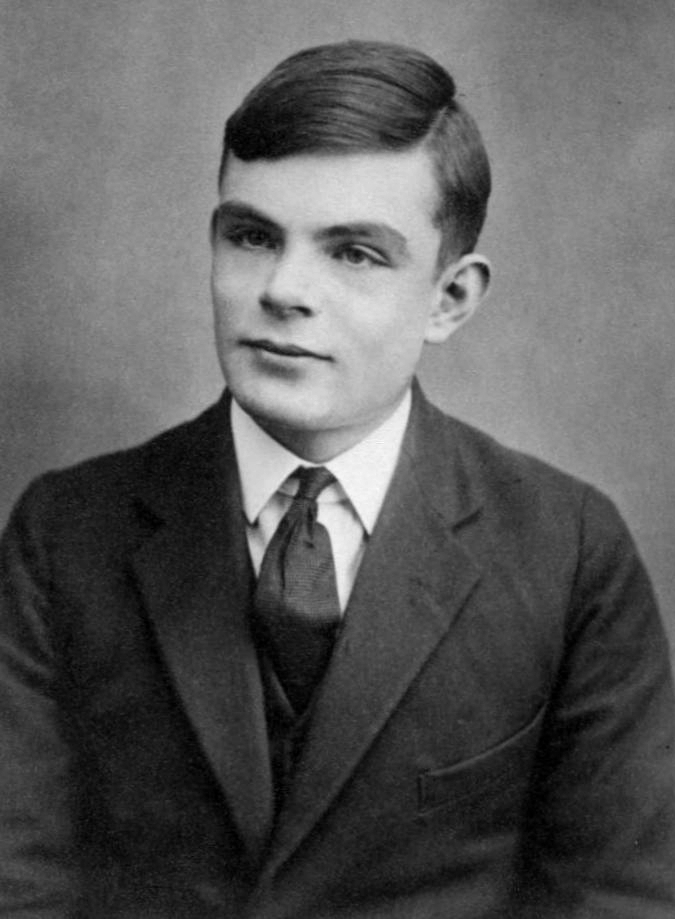
\includegraphics[width=1.0in]{images/turing.jpg}}
\caption*{\small ``A function is said to be `effectively calculable' if its
values can be found by some purely mechanical process.'' -- Alan Turing,
\href{https://doi.org/10.1112/plms/s2-45.1.161}{\emph{Systems of Logic Based
on Ordinals}} (1939), p.~166.}
\end{figure}

\begin{figure}[ht]
\centerline{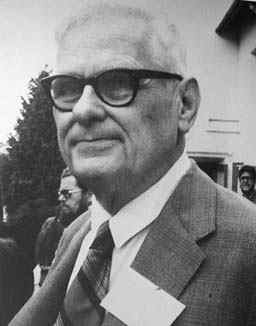
\includegraphics[width=1.0in]{images/church.jpg}}
\caption*{\small ``a function of positive integers shall be called
effectively calculable if it is recursive'' -- Alonzo Church,
\href{https://phil415.pbworks.com/f/Church.pdf}{\emph{An Unsolvable Problem
of Elementary Number Theory}} (1936), p.~346, footnote~3 (excerpt).}
\end{figure}

The agreement of these independently developed models gives us confidence
that they capture the informal idea of calculation by explicit, mechanical
rules. The assertion that they encompass \emph{every effective mechanical
procedure} is the \emph{Church--Turing thesis}. Unlike the equivalence of
the formal models, this assertion is not a mathematical theorem: it connects
a precise mathematical definition with an informal idea. In Church's
quotation, ``recursive'' includes the possibility of unbounded search;
primitive recursion alone would not suffice. We need no knowledge of the
other models to use ours. Its scope concerns what can be computed, not
whether every procedure we write terminates or gives the intended answer.




\section*{Problems}
\begin{enumerate}
\item Unfold $\operatorname{add}(2,4)$ and $\operatorname{fact}(5)$.
Mark the operations that are deferred. Trace the corresponding tail-recursive
computations and identify their states.
\item State the induction hypothesis for division and remainder using the
quotient $q$. Explain why using $q$ in the proof does not require knowing
it before running the algorithm.
\item Trace quotient and remainder for $(23,4)$. Define a tail-recursive
function that computes both together, using a remainder candidate and a
quotient accumulator. State and prove its invariant.
\item Trace $G(105,252)$. Explain why an initial assumption $a\geq b$ is
unnecessary, and why the second argument is a suitable termination measure.
\item Prove that $5n^2+3n+8=O(n^2)$. Explain why an $O(n^2)$ upper bound
alone does not establish that an algorithm needs quadratic time.
\item Compare the number of multiplications for $3^{16}$ using
$\operatorname{pow}$ and $E$, following the definitions exactly. Explain
what happens if $\operatorname{sqr}$ is replaced by two independently
evaluated recursive calls.
\item Explain how the invariant for $F(k,p)$ determines its next state. Describe which value must be used
in the multiplication if the two components of its state are updated one
at a time.
\item Under the hypothetical rate of $10^9$ steps per second, estimate the
time for $2^{60}$ steps. How much does a thousandfold speed-up increase the
input size possible in a fixed time? Compare with an algorithm taking $n^2$
steps.
\item For $f(i)=2i+1$, unfold $\operatorname{Sum}_f(1,3)$ and trace
$J_f(1,3,0)$. Check the invariant at each state, and state the addition-count
recurrence. What changes if one evaluation of $f(i)$ costs $i$ steps?
\item Prove the upper bound for fast power by induction using its recurrence.
Explain why counting one recursive call instead of two is decisive.
\item In Euclid's algorithm, show that two consecutive positive remainders
cannot both exceed half the earlier second argument. Use this to derive
a logarithmic bound without assuming anything about Fibonacci numbers.
\item Explain why ``no successful candidate at most $B$'' does not usually
mean ``no successful candidate exists''. What extra fact makes a bounded
search sufficient in the square-root example?
\item Explain why the unbounded search for a square root may fail to halt.
Modify it to return a special failure code when no natural-number square root
exists, and explain why the modified search always terminates.
\item Define recursive and tail-recursive algorithms for
$\prod_{i=a}^{b}f(i)$, with an empty product equal to $1$. Prove the recursive
version correct by induction on the number of factors. Give an invariant
for the iterative version.
\item Let $B(0)=1$ and $B(n)=B(n-1)+B(n-1)$ for $n>0$. Show by induction
on $n$ that $B(n)=2^n$. If the two recursive calls are evaluated separately,
derive the recurrence for the number of additions and solve it. Rewrite the
algorithm to use only $n$ additions.
\item The Fibonacci numbers are $F_0=0$, $F_1=1$, and
$F_{n+2}=F_{n+1}+F_n$. Design an iterative algorithm that starts with
$(i,u,v)=(0,0,1)$ and maintains $u=F_i$, $v=F_{i+1}$. State its stopping
condition, prove correctness, and count its additions.
\item Evaluate $G(34,21)$ and $G(55,34)$. Compare the successive remainders
with the Fibonacci numbers. Explain why each reduction is small compared
with the case in which the smaller input divides the larger exactly.
\item Construct a tail-recursive fast-power algorithm using a state $(b,k,p)$
with invariant $p b^k=x^n$. Start with $(b,k,p)=(x,n,1)$.
What state change works when $k$ is even? What works when it is odd?
Prove that the algorithm terminates and uses logarithmically many
multiplications. State what happens when $n=0$.
\item To count how many values among $f(a),\ldots,f(b)$ are even, define a
recursive algorithm using an if--then--else test. Prove it correct by induction
on the number of terms. Then derive an iterative version and its invariant.
\item Suppose an algorithm has a correct invariant but its state never
changes. Must it return the right answer? Give an example and explain
precisely what an invariant proves and what a termination argument adds.
\end{enumerate}
